%% LyX 2.3.3 created this file.  For more info, see http://www.lyx.org/.
%% Do not edit unless you really know what you are doing.
\documentclass[11pt]{article}
\usepackage[latin9]{inputenc}
\usepackage{url}
\usepackage{mathtools}
\usepackage{graphicx}
\usepackage{subcaption}
\usepackage{listings}

\makeatletter
%%%%%%%%%%%%%%%%%%%%%%%%%%%%%% User specified LaTeX commands.
%Gummi|065|=)
\usepackage{url}
\title{\textbf{Capstone Project}}
\author{Allyson Julian}
\date{February 8, 2020}

\makeatother

\begin{document}
\maketitle

\section{Definition}

\subsection{Project Overview}

Advances in agricultural technology over the past 30 years have made
it easier for farmers to manage their farms, particularly when the
farms are comprised of multiple fields greater than 1000 acres in
size. The use of GPS on aerial imagery, drones, etc. have been instrumental
in precision agriculture \cite{liakos_machine_2018}.

But one of the challenges of modern farming is the detection of plant
diseases. For large farms in particular, it is time-consuming for
a farmer to manually check each growing plant for disease. It can
potentially be more cost-effective to diagnose plant diseases with
automated tools \cite{fujita_basic_2016}.

For this project, I built the Python library \textbf{ikapati} (named after the Filipino goddess of agriculture), which implements a plant disease detector and then deployed the best-performing model to an embedded system built specifically for use in Artificial Intelligence applications, a Jetson Nano robot.	

The library also provides utility tools to do many of the tasks required in machine learning research, including the image preprocessing necessary to prepare the data for classification, scripts to train classifier itself, and utility functions to help evaluate performance.

\subsection{Problem Statement}

The main objective for this project was to build a library that can be used for training a plant disease classifier and in doing so act as a framework with which to do further research in this subject area. It can be used to complete an entire machine learning pipeline from training to deployment to an embedded system.

To build this library, I needed to:

\begin{enumerate}
	\item Retrieve the PlantVillage Dataset (\url{https://github.com/spMohanty/PlantVillage-Dataset}).
	\item Prepare the raw color images from the PlantVillage Dataset for consumption by the model.
	\item Train the model to classify the different diseases for a given species of plant.
	\item Save the model as a TensorFlow Lite object for use in an embedded system.
\end{enumerate}

\subsection{Metrics}

Accuracy and loss were the main metrics used in this project to evaluate overall model performance. 

Accuracy is generally defined as such:

\begin{equation}
\frac{TP + TN}{TP + TN + FP + FN}
\end{equation}

Where $TP$ = true positives, $TN$ = true negatives, $FP$ = false positives, $FN$ = false negatives.

Validation and training loss was used to determine whether the model was overfitting, underfitting, or fitting adequately. 

If the curve of the validation loss decreases until a certain point, and then starts to increase again, it is indicative of overfitting.

If the curve of the training loss remains flat then the model may be underfit.
 
\clearpage
\section{Analysis}

\subsection{Data Exploration}

The main datasets used were obtained from the PlantVillage Dataset: \url{https://github.com/spMohanty/PlantVillage-Dataset}

The dataset consists of 52,803 JPEG images with the dimensions 256x256. All of the images are colored, so there are 3 channels corresponding to the RGB mode.

The images are cropped in such a way that the leaves are centered in the picture, and have a fairly uniform-looking, solid background.

The images are split up into several folders, labelled according to the plant species (e.g. Peach) and disease class (e.g. Bacterial spot).

\begin{figure}[h!]
  \centering
  \begin{subfigure}[b]{0.3\linewidth}
    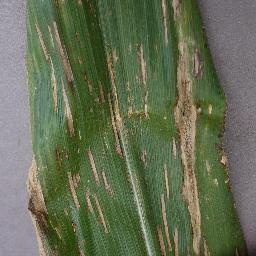
\includegraphics[width=\linewidth]{figures/examples/corn.jpg}
    \caption{Corn leaf spot}
  \end{subfigure}
   \begin{subfigure}[b]{0.3\linewidth}
    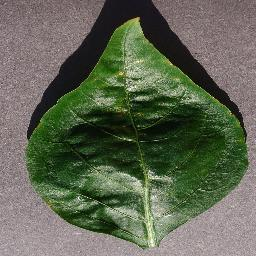
\includegraphics[width=\linewidth]{figures/examples/pepper.jpg}
    \caption{Pepper}
  \end{subfigure}
   \begin{subfigure}[b]{0.3\linewidth}
    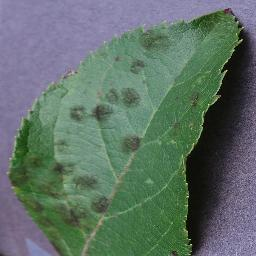
\includegraphics[width=\linewidth]{figures/examples/scab.jpg}
    \caption{Apple Scab}
  \end{subfigure}
  \caption{Example images in dataset.}
  \label{fig:benchmark}
\end{figure}

Further data exploration can be viewed in the 1.0-agj-data-exploration.ipynb notebook.

\subsection{Algorithms and Techniques}

A \textbf{Convolutional Neural Network (CNN)} was selected as the classification algorithm due to its demonstrated efficacy in plant disease detection in previous studies \cite{toda_how_2019} \cite{fujita_basic_2016}.

Two CNN architectures were used in this project:

\begin{enumerate}
	\item is based on \textbf{AlexNet} \cite{krizhevsky_imagenet_2017} and is comprised of Conv2D (which does convolution), MaxPooling2D (max pooling), and FCD (which are a combination of Dense and Dropout layers).
	\item is based on the \textbf{InceptionV3} based network built in the study by Toda et al \cite{toda_how_2019} that demonstrated an accuracy of 99.99\% in predicting plant disease classification on the PlantVillage Dataset.
\end{enumerate}

\subsubsection{AlexNet}

This describes the layer sequence (the number indicates how many of that same layer repeats until the next one):

\begin{itemize}
	\item Conv2D (3) - Convolution Layer
	\item MaxPooling2D (1) - Max Pooling Layer
	\item Conv2D (2) - Convolution Layer
	\item MaxPooling2D (1) - Max Pooling Layer
	\item FCD (3) - Fully Connected Layer w/ optional Dropout.
\end{itemize}


\begin{figure}[h!]
	\centering
	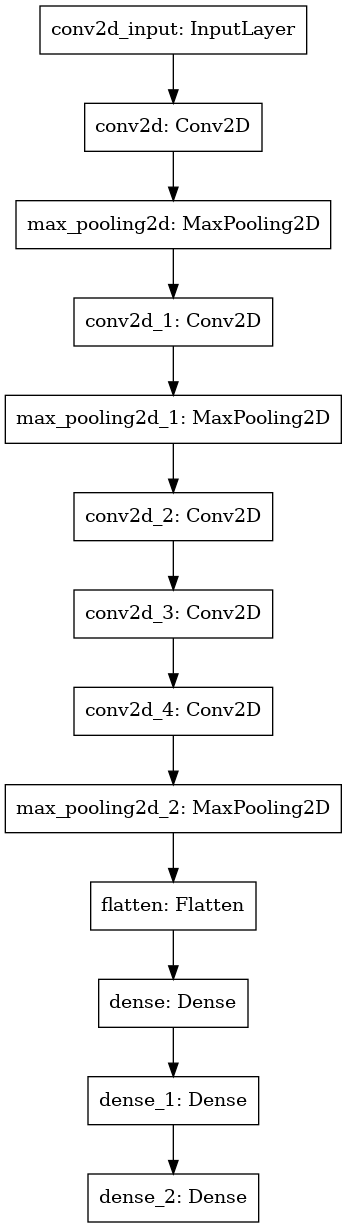
\includegraphics[width=0.2\linewidth]{figures/alexnet.png}
    \caption{AlexNet Architecture}
  	\label{fig:alexnet}
\end{figure}


\subsubsection{InceptionV3}

This InceptionV3-based network is based on what was done in a previous study \cite{toda_how_2019}, but as 10 Mixed modules instead of the 11 used in that study.

\begin{itemize}
	\item Conv2D (3) - Convolution Layer with Batch Normalization
	\item MaxPooling2D (1) - Max Pooling Layer
	\item Conv2D (2) - Convolution Layer with Batch Normalization
	\item MaxPooling2D (1) - Max Pooling Layer
	\item Mixed (10) - Sets of Conv2D with batch normalization
	\item GlobalAveragePooling2D (1) - Global Pooling Layer
	\item Dense (1) - The Output Layer
\end{itemize}

See \textbf{Additional Figures} to view visualization of InceptionV3.
 
\subsubsection{Hyperparameters}

These parameters can be tuned/specified at training time:

\begin{itemize}
	\item \textbf{epochs} - the number of times to run through the training set.
	\item \textbf{learning rate} - the learning rate for the Adam optimizer.
	\item \textbf{batch size} - the number of training examples in each batch.
	\item \textbf{activation} - the activation function to use, e.g. "relu".
	\item \textbf{dropout} - the dropout rate, e.g. 0.2. This was only supported by AlexNet.
	\item \textbf{architecture} - the architecture to use for the CNN, "alexnet" (for AlexNet) or "inceptionv3" (for InceptionV3).
\end{itemize}

\subsection{Benchmark}

The benchmark for the plant disease classifier are results obtained by previous studies by
Toda et al, Fuentes et al, on plant detection which all utilize a CNN as a classifier\cite{toda_how_2019} \cite{fuentes_robust_2017}.

\newpage
\section{Methodology}

\subsection{Data Preprocessing}

Preprocessing the data was completed using these steps:

\begin{enumerate}
	\item Get a list of all image filenames.
	\item Shuffle list of image filenames. 
	\item Get labels from the image folder names. For example: images that were in the Apple\_\_\_Apple\_scab were assigned the label Apple\_\_\_Apple\_scab.
	\item Split list of image filenames into training files (60\%), validation (20\%), and testing files (20\%) to mirror the split in a previous study \cite{toda_how_2019} .
	\item Create a training example for each image file so it can be added to a TFRecord (TensorFlow dataset).
	\item Write metadata describing the file counts of training, validation, and test sets and list the class names.
	\item Create parser function to read each TFRecord batch by batch during training due to hardware limitations (limited VRAM, in this case).
	\item Normalize image pixel values by dividing by 255 (representing the range of values for an RGB image) and subtract -0.5 to the values to make them fall in the -0.5 to 0.5 range.
\end{enumerate}

\subsection{Implementation}

The library was primarily written in Python 3. TensorFlow 2.0 with the keras API was used in the training stage.

The modules for the \textbf{ikapati} library can be broken down as such:

\begin{itemize}
	\item \textbf{models} - these contain the training script and code to build the networks.
	\item \textbf{data} - this has the utility functions used to preprocess the data, e.g. normalizing pixel values, reading datasets into memory.
	\item \textbf{visualization} - this contains utility functions to help visualize and evaluate model performance. Figures included in this report were generated using that module.
\end{itemize}

\subsubsection{Data Preparation}

The datasets were prepared using the \textbf{ikapati/data/make\_dataset.py} script (which utilizes datasets scikit-learn and TensorFlow 2.0) and then saved as TFRecords, a format used by TensorFlow.

\begin{enumerate}
	\item Get the filenames of all the images that match the specified plant species.
	\item Follow the steps outlined in the \textbf{Data Preprocessing} section.
	\item Put each subset of training examples (training, validation, and test) into separate TFRecords (train.tfrecord, eval.tfrecord, test.tfrecord).
\end{enumerate}

\subsubsection{Training Stage}

The training models were created using TensorFlow 2.0 with the keras functional API. As described in the section \textbf{Algorithms and Techniques}, CNN was chosen as the classifier, with neural network architectures based on AlexNet and InceptionV3 as described in a previous study \cite{toda_how_2019} . TensorFlow was configured to use a physical GPU similar to what was used in the Toda study, a GeForce GTX 1080 Ti with 11GB of VRAM, to do the training.

The code used to build the AlexNet architecture was based on:

\begin{itemize}
    \item \url{https://engmrk.com/alexnet-implementation-using-keras/}
	\item \url{https://github.com/tensorpack/benchmarks/blob/master/other-wrappers/keras.alexnet.py}
\end{itemize}

The code used to build the InceptionV3 architecture was based on:

\begin{itemize}
    \item \url{https://github.com/keras-team/keras-applications/blob/master/keras_applications/inception_v3.py}
\end{itemize}

The training steps for each training run were:

\begin{enumerate}
	\item Execute the ikapati/models/train\_model.py script with the architecture (alexnet or inceptionv3), learning rate, epochs, batch size, activation, and dropout rate (if architecture is set to alexnet) hyperparameters specified, the model and data directories set, and checkpoint saving enabled to kick off a training run. (See the \textbf{Hyperparameters} described in the section \textbf{Algorithms and Techniques} for more details on the hyperparameters).
	\item Create a folder under the model dir specified at runtime, with the UUID of dataset used as the name, and a subfolder within that with the start time string as the name. This will be where the models are saved during this training run.
	\item Record the start time.
	\item After each epoch, if the validation loss has improved from the previous epoch, save the model to file in h5 format. Otherwise, we don't save anything and proceed with the next epoch.
	\item When all epochs have concluded, save the final model to file and record the end time.
	\item Write the start and end time of the training run, the learning rate, and other parameters specified at runtime to a CSV file that acts as a log of training runs.
	\item Repeat steps above, tweaking the hyperparameters as needed.
\end{enumerate}

\subsection{Refinement}

In the initial benchmark run, the hyperparameters were set to match that of the benchmark model from Toda et al, with the learning rate set to 0.05, the batch size to 128, and the epochs to 20. The architecture was inceptionv3 and the activation function was "relu" (rectified linear units). \textbf{NOTE} The benchmark model input shape was 224x224, where as in this project the input shape was 256x256.

The benchmark model achieved an accuracy of 85.68\% on the test dataset, and a loss score of 0.570 (Figure ~\ref{fig:benchmark}). 

\begin{figure}[h!]
  \centering
  \begin{subfigure}[b]{0.6\linewidth}
    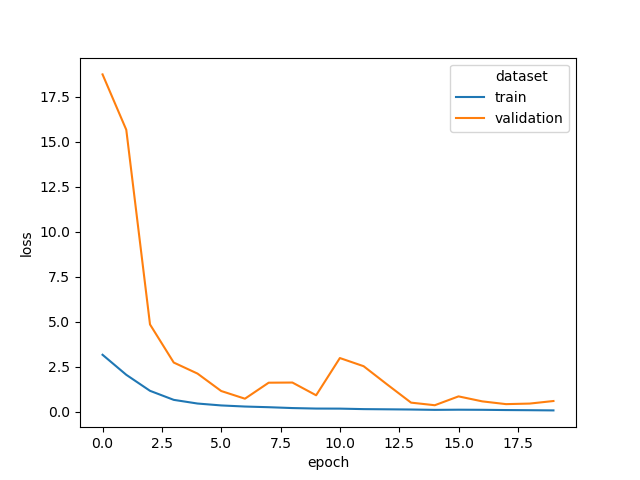
\includegraphics[width=\linewidth]{figures/benchmark-loss.png}
    \caption{Training vs Validation Loss}
  \end{subfigure}
  \begin{subfigure}[b]{0.6\linewidth}
    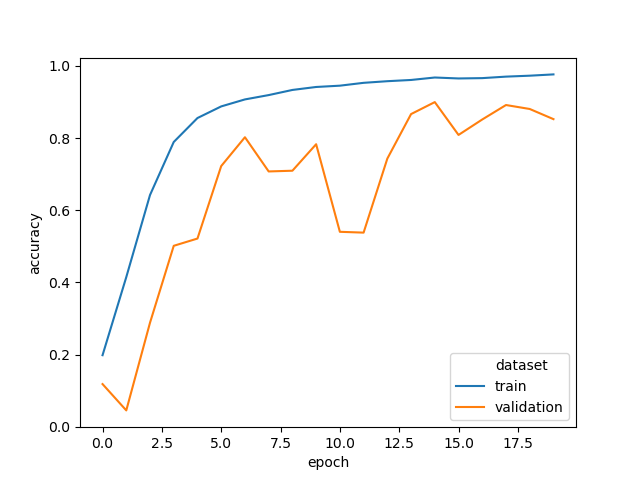
\includegraphics[width=\linewidth]{figures/benchmark-accuracy.png}
    \caption{Training vs Validation Accuracy}
  \end{subfigure}
  \caption{Loss and accuracy plots for the benchmark model.}
  \label{fig:benchmark}
\end{figure}

In subsequent training runs, certain modifications were made to the hyperparameters to see if it would improve the model validation loss and accuracy:

\begin{itemize}
	\item The learning rate was decreased to 0.001.
	\item The batch size was reduced to account for hardware limitations.
	\item The epoch number was increased to see if the model's validation loss decreases over time.
	\item If validation loss improved in one epoch, then a checkpoint of the model was saved to file.
	\item After each iteration, the validation vs training loss was plotted to determine whether a model is underfitting or overfitting, or reaching a good fit.
	\item When selected as the architecture, AlexNet demonstrated a tendency to overfit on this dataset even with dropout layers, so InceptionV3 became the defacto architecture. 
\end{itemize}

\subsubsection{Visualization and Metrics Tools}

Utility functions to evaluate model performance were created using seaborn (a high-level API for matplotlib) and pandas.

\subsubsection{Deployment to an Embedded System}

Upon training completion, trained models as saved in both h5 and tflite (TensorFlow Lite) formats. Both formats can be loaded for later use with the TensorFlow library, but the tflite format is specifically used to run inference on embedded devices such as the Jetson Nano mentioned previously.

A simple web app was created using the Flask framework. 

This web app has a POST endpoint located at \url{http://jetbot:5000/predict}, which loads the tensorflow lite model and then attempts to predict the class name for an input image uploaded using that endpoint.

To simulate a POST request to that endpoint, the curl commandline tool was used with the image file passed in:

\begin{lstlisting}
curl -F "image=@blight.jpg" http://jetbot:5000/predict
\end{lstlisting}

This endpoint expects a 256x256 image. If the request is successful, the result will be a JSON body containing the predicted class for the input image:

\begin{lstlisting}
{
  "class_name": "Tomato___Septoria_leaf_spot"
}
\end{lstlisting}

\clearpage
\section{Results}

\subsection{Model Evaluation and Visualization}

Model performance was evaluated with accuracy and loss plots (Figure ~\ref{fig:best1}). 

Models that showed overfitting, such as the AlexNet-based model, were discarded.

\begin{figure}[h!]
  \centering
  \begin{subfigure}[b]{0.6\linewidth}
    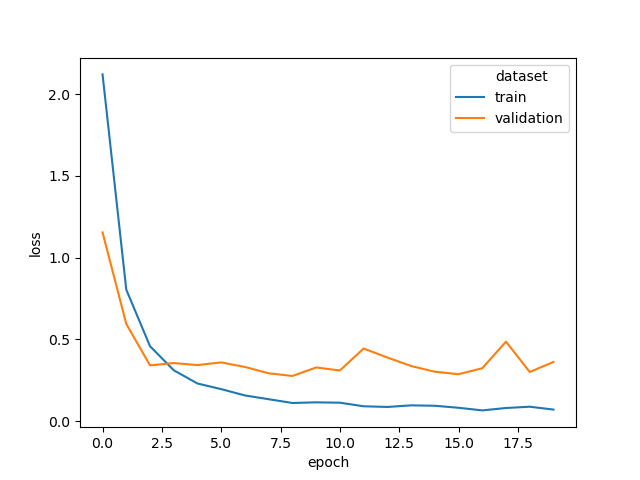
\includegraphics[width=\linewidth]{figures/alexnet-loss.png}
    \caption{Training vs Validation Loss}
  \end{subfigure}
  \begin{subfigure}[b]{0.6\linewidth}
    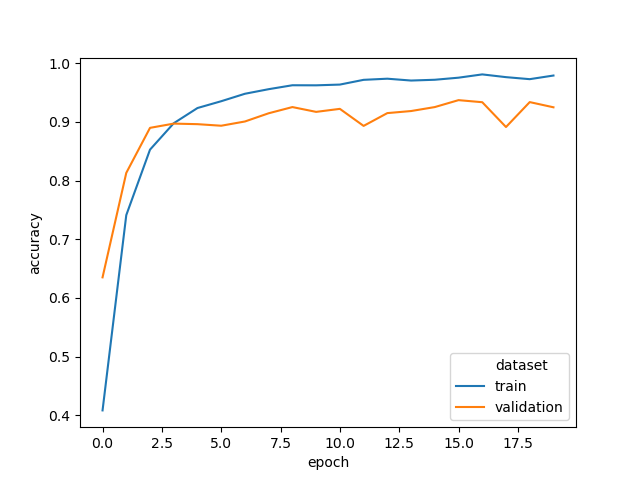
\includegraphics[width=\linewidth]{figures/alexnet-accuracy.png}
    \caption{Training vs Validation Accuracy}
  \end{subfigure}
  \caption{Loss and accuracy plots for AlexNet. Validation shows overfitting.}
  \label{fig:alexnet}
\end{figure}

The 2 best performing models, based on these metrics, were both InceptionV3-based and outperformed the benchmark. In both of these runs, the learning rate was reduced to 0.001 from the benchmark 0.05.

\begin{figure}[h!]
  \centering
  \begin{subfigure}[b]{0.6\linewidth}
    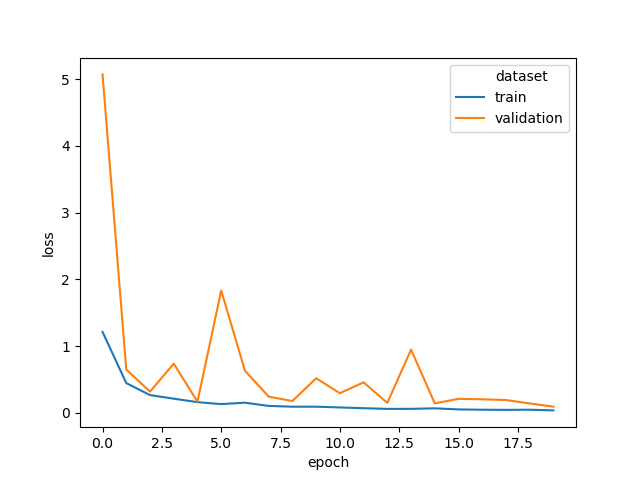
\includegraphics[width=\linewidth]{figures/best-model-loss-4632.png}
    \caption{Training vs Validation Loss}
  \end{subfigure}
  \begin{subfigure}[b]{0.6\linewidth}
    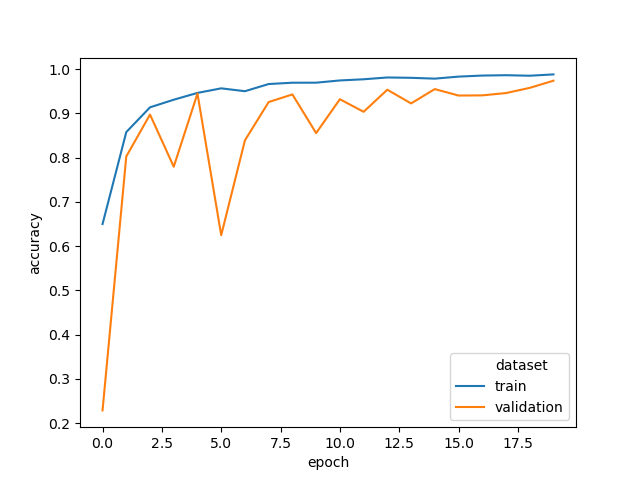
\includegraphics[width=\linewidth]{figures/best-model-accuracy-4632.png}
    \caption{Training vs Validation Accuracy}
  \end{subfigure}
  \caption{Model 1. Loss and accuracy plots for InceptionV3, with batch size of 64 and learning rate of 0.001.}
  \label{fig:best1}
\end{figure}

\begin{figure}[h!]
  \centering
  \begin{subfigure}[b]{0.6\linewidth}
    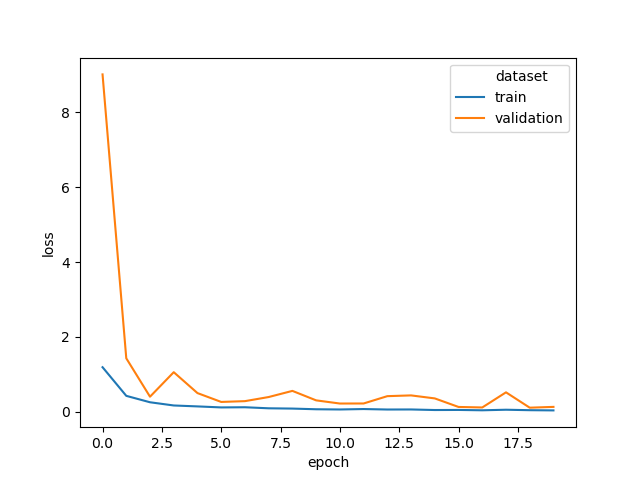
\includegraphics[width=\linewidth]{figures/best-model-loss-5614.png}
    \caption{Training vs Validation Loss}
  \end{subfigure}
  \begin{subfigure}[b]{0.6\linewidth}
    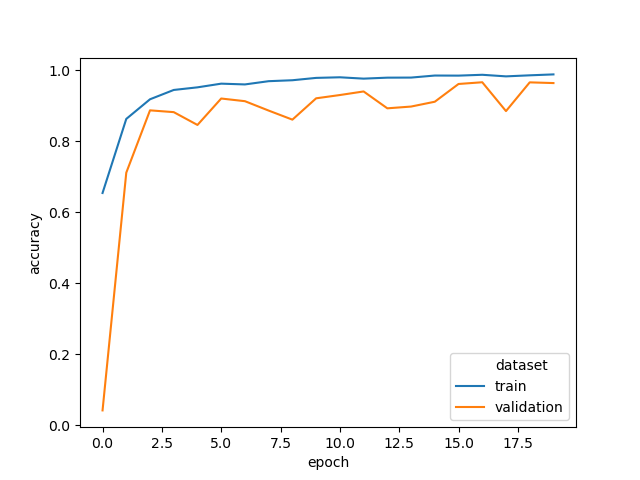
\includegraphics[width=\linewidth]{figures/best-model-accuracy-5614.png}
    \caption{Training vs Validation Accuracy}
  \end{subfigure}
  \caption{Model 2. Loss and accuracy plots for InceptionV3, with batch size of 100 and learning rate of 0.001.}
  \label{fig:best2}
\end{figure}

In Figure ~\ref{fig:best1}, the plots show how that training run Model 1, with the batch size reduced to 64 from 128 performed on the validation and training sets. On the test dataset, this model performed with an accuracy of 97\% and a loss score of 0.089.

In Figure ~\ref{fig:best2}, the plots show how the training run with the same batch size as the benchmark but a learning rate reduced to 0.001 performed. On the test dataset, this this model performed with an accuracy of 96\% and a loss score of 0.126.

While Model 1 and 2 performed similarly, Model 1 did better on the test dataset than Model 2, so it was selected as the Best Model.

\subsection{Justification}

The Best Model was converted to TensorFlow Lite format (tflite) and then transferred to the 

\clearpage
\section{Conclusion}

\subsection{Free-Form Visualization}

\begin{figure}[h!]
  \centering
  \begin{subfigure}[b]{0.5\linewidth}
    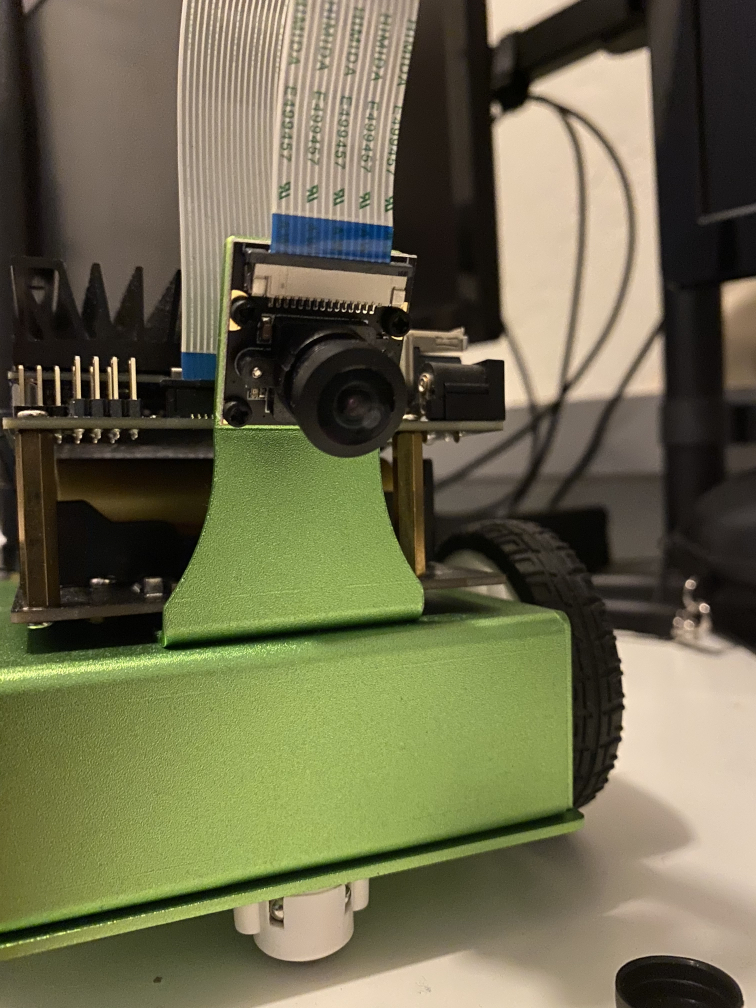
\includegraphics[width=\linewidth]{figures/IMG_7846.jpg}
    \caption{Jetson Nano Robot with Camera}
  \end{subfigure}
  \begin{subfigure}[b]{0.5\linewidth}
    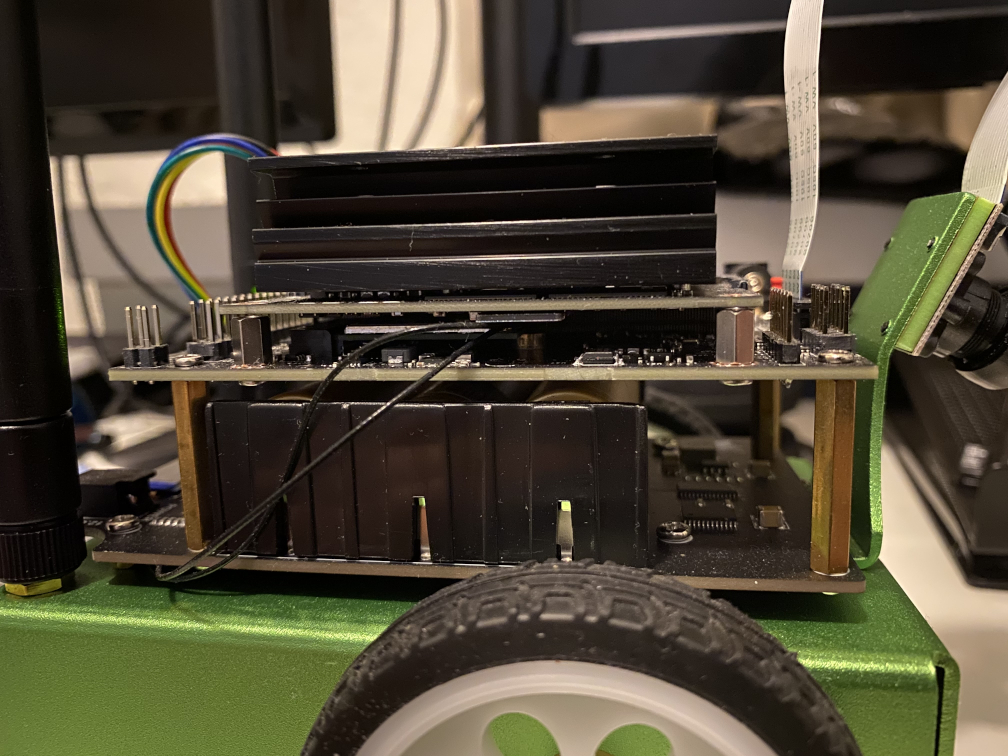
\includegraphics[width=\linewidth]{figures/IMG_7845.jpg}
    \caption{Side view of the Jetson Nano Robot}
  \end{subfigure}
  \caption{Jetson Nano Robot}
  \label{fig:jetson}
\end{figure}

\subsection{Reflection}

These steps summarize what was done to complete this project:

\begin{enumerate}
	\item Initial exploration of the agricultural domain was done to see what problems need more investigation.
	\item A large dataset with multiple classes of plants was downloaded and then preprocessed.
	\item A benchmark model was created based on a previous study \cite{toda_how_2019} .
	\item Models built in TensorFlow were trained using different hyperparameters and 2 different architectures.
	\item The best model was chosen using validation loss and accuracy scores and then converted to TensorFlow Lite format.
	\item A simple Flask API that loads the TensorFlow Lite model and does inference, was deployed to a Jetson Nano.
\end{enumerate}

I found 3-4, and 6 most challenging because I had never used TensorFlow at the level this project required and had never built a CNN before.

It was interesting to learn about how those neural networks work and how they can be improved upon.

\subsection{Improvement}

There is some opportunities for improvement from this project:

\begin{itemize}
	\item The dataset used here consisted of pictures with leaves that were set against a fairly uniform background. In a future iteration of this project, the dataset could be augmented by introducing random noise and transformations to a subset of images, and then use that to train.
	\item The machine learning model could be converted to do online learning so that learning can be done as inference is attempted. This could be especially useful when trying to improve the accuracy of the model.
	\item 
\end{itemize}

\clearpage
\bibliographystyle{IEEEtran}
\bibliography{citations}
	
\end{document}

